\section{Consenso con Seguimiento de Líder}
\onecolumn
\subsection{Líder con metas secuenciales}
Se introduce un líder que recorre una ruta de metas. Los seguidores hacen consenso entre sí y son atraídos hacia la posición actual del líder, no hacia la meta:
\begin{align*}
    \dot{\mathbf{x}}_i &= \mathbf{u}_i \\[6pt]
    \mathbf{u}_i &=
    \underbrace{\sum_{j \in \mathcal{N}_i} a_{ij}\,(\mathbf{x}_j-\mathbf{x}_i)}_{\text{\footnotesize Consenso entre seguidores}}
    \;\;
    \underbrace{+\,\beta\, b_i^0\,(\mathbf{x}_0-\mathbf{x}_i)}_{\text{\footnotesize Atracción al líder}}
\end{align*}

\section{Consenso con Seguimiento de Líder}
\onecolumn
\subsection{Líder con metas secuenciales}
El líder $\mathbf{x}_0$ avanza hacia cada meta con control proporcional, desplazando el valor de consenso del grupo hacia una referencia móvil.

\begin{figure}[H]
    \centering
    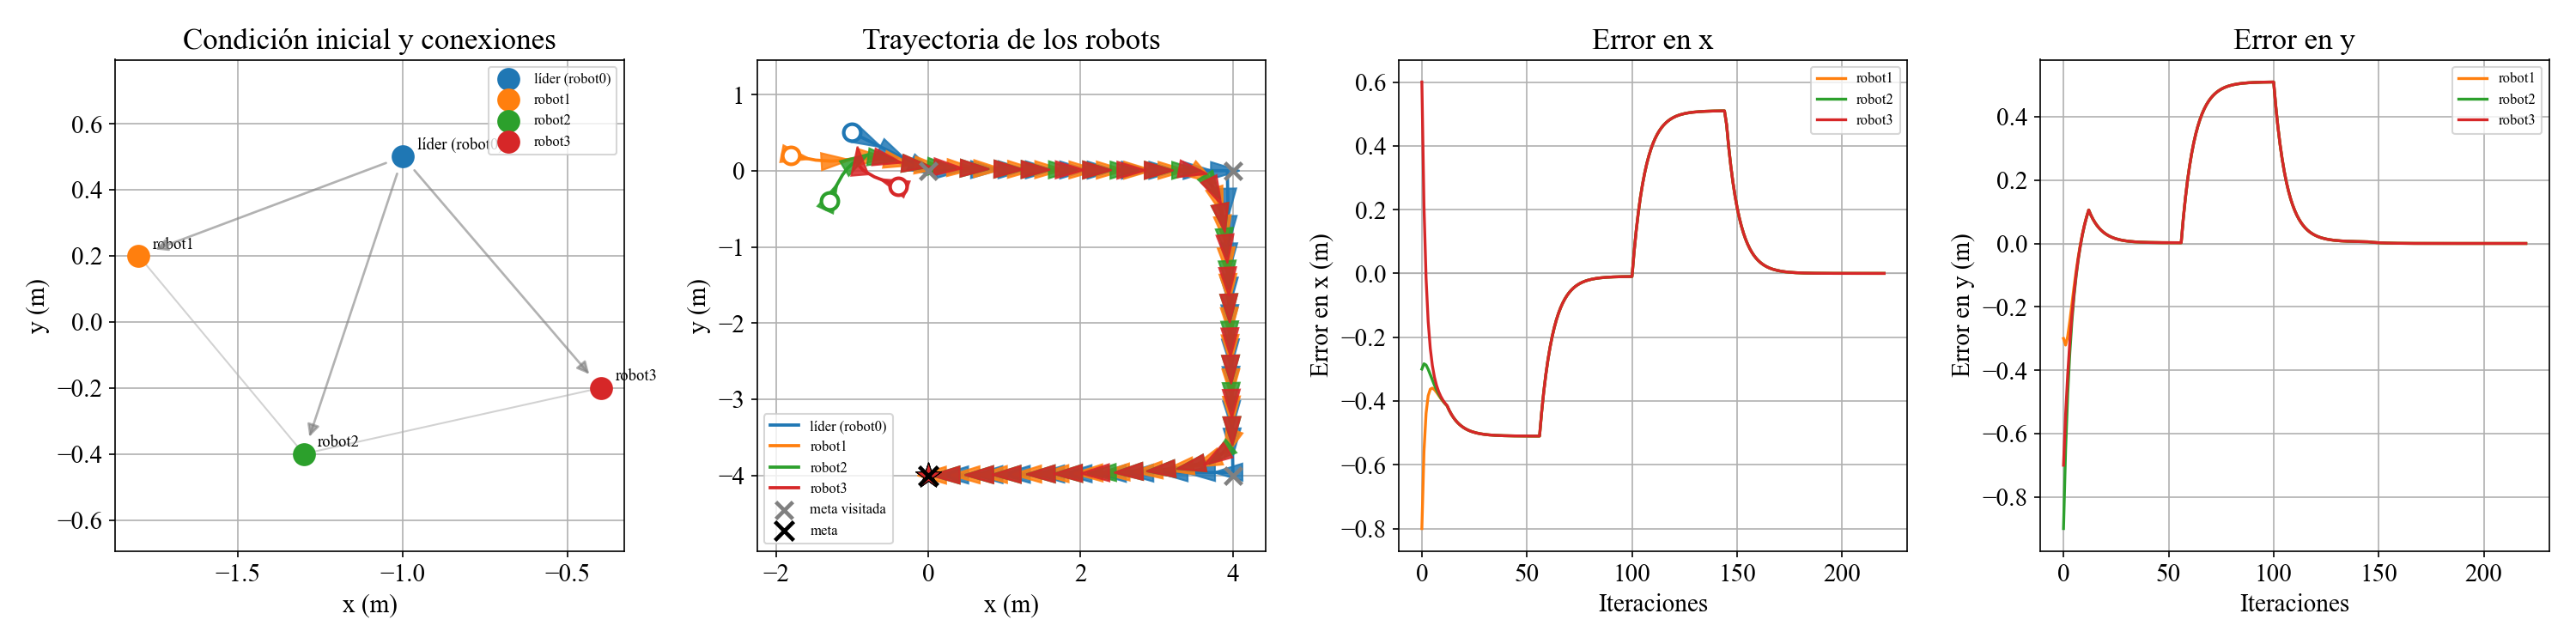
\includegraphics[width=\linewidth]{Pics/lider_seguidor_multimeta_mid3 (1).png}
    \caption{El líder recorre cuatro metas secuenciales mientras los seguidores lo persiguen manteniendo el consenso entre sí.}
    \label{fig:lider_seguidor}
\end{figure}
